\section{Результати з англійської мови}

Оглянемо отримані $78\ 797$ результатів, де жіночих є на $8\ 339$ більше за чоловічих. Зобразимо гістограми результатів ЗНО з англійської мови 2019 року для вибірки, наприклад, $10\ 000$ учнів:

\begin{figure}[H]
    \center{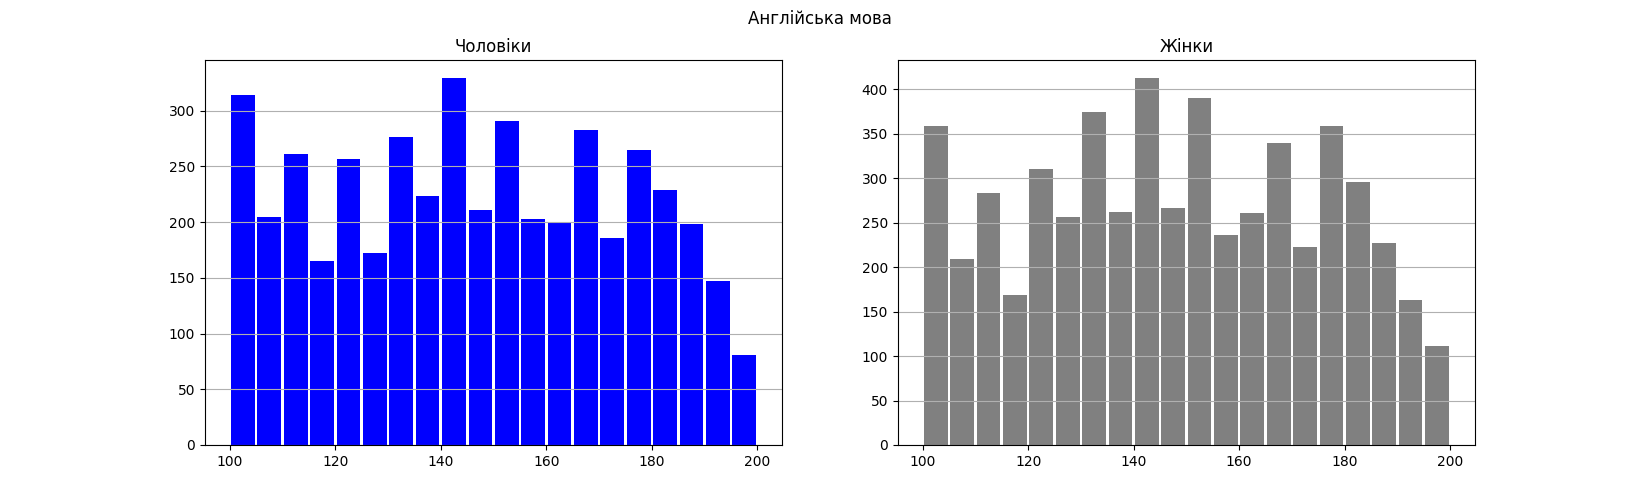
\includegraphics[trim=4cm 0cm 4cm 1cm, clip, width=1\linewidth]{ENG figures/ENG_10000.png}}
    \caption{Результати з англійської мови}
    \label{figure: ENG initial data}
\end{figure}

З'ясуємо, чи відмінність між результатами для жінок та чоловіків є статистично значущою.

\subsection{Перевірка гіпотези однорідності даних}

Нехай маємо дві незалежні вибірки $\left\{ X_i \right\}$ та $\left\{ Y_j \right\}$ однаково розподілених  випадкових величин, розподіли $F_x$ й $F_y$ яких нам невідомі:
\begin{align*}
    &X_1 \ldots X_n\sim F_x && \text{результати чоловіків} \\
    &Y_1 \ldots Y_m\sim F_y && \text{результати жінок}
\end{align*}

Перевіримо гіпотезу про однорідність статистичного матеріалу, тобто гіпотезу, що ймовірності 
спостереження умовно високих, помірних та низьких балів в обох вибірках є однаковими. Таким чином 
матимемо $k=2$ вибірок, в яких елементи приймають $s=3$ різних значень. Знову за аналогічних позначень гiпотеза перевiрки однорiдностi спосережуваних даних формулюватиметься так само як і у виразах~(\ref{formula: hypothesis}):
\begin{align*}
    &\text{нульова гіпотеза} &&H_0: p_{11}=p_{21},\ p_{12}=p_{22},\ p_{13}=p_{23} \\
    &\text{проти альтернативи} && H_1: \exists i,j\quad p_{1,j}\neq p_{2,j}
\end{align*}

А тоді критерієм перевірки гіпотези рівно як і у випадку обробки результатів з 
української мови (\ref{formula: criterion}) слугуватиме правило
\begin{equation*}
    \delta(x_1\ldots x_n,\ y_1\ldots y_m)=
    \begin{cases}
        H_1, & \rho\geqslant\chi^2_{1-\alpha;\ (k-1)(s-1)} \\
        H_0, & \rho<\chi^2_{1-\alpha;\ (k-1)(s-1)} \\
    \end{cases}
\end{equation*}

При цьому статистика критерію $\rho$ обчислюється аналогічно до формули (\ref{formula: criterion statistics}):
\begin{equation*}
    \rho\equiv \rho(x_1\ldots x_n,\ y_1\ldots y_m)=(n+m)\left( \sum\limits_{i=1}^k \sum\limits_{j=1}^s 
    \frac{\vartheta_{ij}^2}{\vartheta_{i\cdot}\vartheta_{\cdot j}} - 1\right)
\end{equation*}

\subsubsection{Таблиця спостережуваних даних}

Зобразимо дані для навмання обраних $n=500$ та $m=500$ елементів із вибірок результатів ЗНО з англійської мови для чоловіків та жінок:

\begin{table}[H]
    \vspace*{0.8cm}
    \begin{center}
        \begin{tabular}{|c||c|c|c|c|}
            \hline
             & \text{Низькі бали} & \text{Помірні бали} & \text{Високі бали} & \text{Всього} \\
            \hline \hline
            \text{Чоловіки} & 248 & 168 & 84 & 500 \\
            \hline
            \text{Жінки} & 224 & 196 & 80 & 500 \\
            \hline
            \text{Всього} & 472 & 364 & 164 & 1000 \\
            \hline
        \end{tabular}
        \caption{Таблиця спостережуваних значень з англійської мови}
        \label{table: ENG homogeneity data}
    \end{center}
\end{table}

Обчислимо значення статистики критерію:
\begin{equation*}
    \rho = 1000\left( \frac{228^2}{472\cdot 500}+\frac{168^2}{364\cdot 500} + \ldots + 
    \frac{196^2}{364\cdot 500}+\frac{80^2}{164\cdot 500} - 1 \right) = 3.47
\end{equation*}

Водночас на рівні значущості $\alpha=0.01$ значення критичної точки
\begin{equation*} 
    \chi^2_{1-\alpha;\ (k-1)(s-1)}=\chi^2_{0.99;\ (2-1)(3-1)}=\chi^2_{0.99;\ 2}=9.21
\end{equation*}

\subsubsection{Висновок}

Оскільки значення статистики критерію є меншим за значення критичної точки, то згідно критерію гіпотеза 
про однорідність статистичних даних приймається. Отже, ймовірності спостереження оцінок різного рівня у 
вибірках для чоловіків та жінок, відповідно, є однаковими. Тобто так само, як і у випадку результатів з 
математики, стать ніяким чином не впливає на рівень отриманого балу.

\subsubsection*{Значення \texttt{p-value}}

Нехай випадкова величина $\tau$ має такий самий розподіл, як і статистика критерію й при цьому не залежить 
від неї: $\tau\sim\chi^2(2)$. Тоді величина \texttt{p-value} обчислюється як така ймовірність:
\[ P(\tau>\rho\ |\ H_0)=P(\tau>3.47)=1-P(\tau\leqslant3.47)=1-F_{\tau}(3.47)=0.1764 \]

Тож для довільних значень $\alpha<\texttt{p-value}$ гіпотеза $H_0$ приймається.

\subsection{Перевірка гіпотези рівності дисперсій}

Для заданих незалежних вибірок $\left\{ X_i \right\}$ та $\left\{ Y_j \right\}$ 
однаково розподілених випадкових величин, розподіли $F_x$ й $F_y$ яких нам невідомі:
\begin{align*}
    &X_1 \ldots X_n\sim F_x && \text{результати чоловіків} \\
    &Y_1 \ldots Y_m\sim F_y && \text{результати жінок}
\end{align*}

Проведемо нормалізацію даних крок за кроком, як це зображено на схемі (\ref{formula: normalization scheme}) 
розділу <<Нормалізація даних>>. У результаті отримаємо такі знормовні вибірки:
\begin{align*}
    &\overline{X^1}\ldots \overline{X^N}\sim N(\mu_x,\tfrac{1}{n}\sigma_x^2) && \text{середні результати чоловіків,} \\
    &\overline{Y^1}\ldots \overline{Y^N}\sim N(\mu_y,\tfrac{1}{n}\sigma_y^2) && \text{середні результати жінок,}
\end{align*}

при цьому
\[ \overline{X^i}=\frac{1}{n}\sum\limits_{j=1}^nX_j,\ 
   \overline{Y^i}=\frac{1}{n}\sum\limits_{j=1}^nY_j,\ i=\overline{1,N} \]

Побудуємо гістограми отриманих вибірок та переконаємося, що вони справді мають нормальний розподіл (Рис. 
\ref{figure: ENG means data}). 

\begin{figure}[H]
    \center{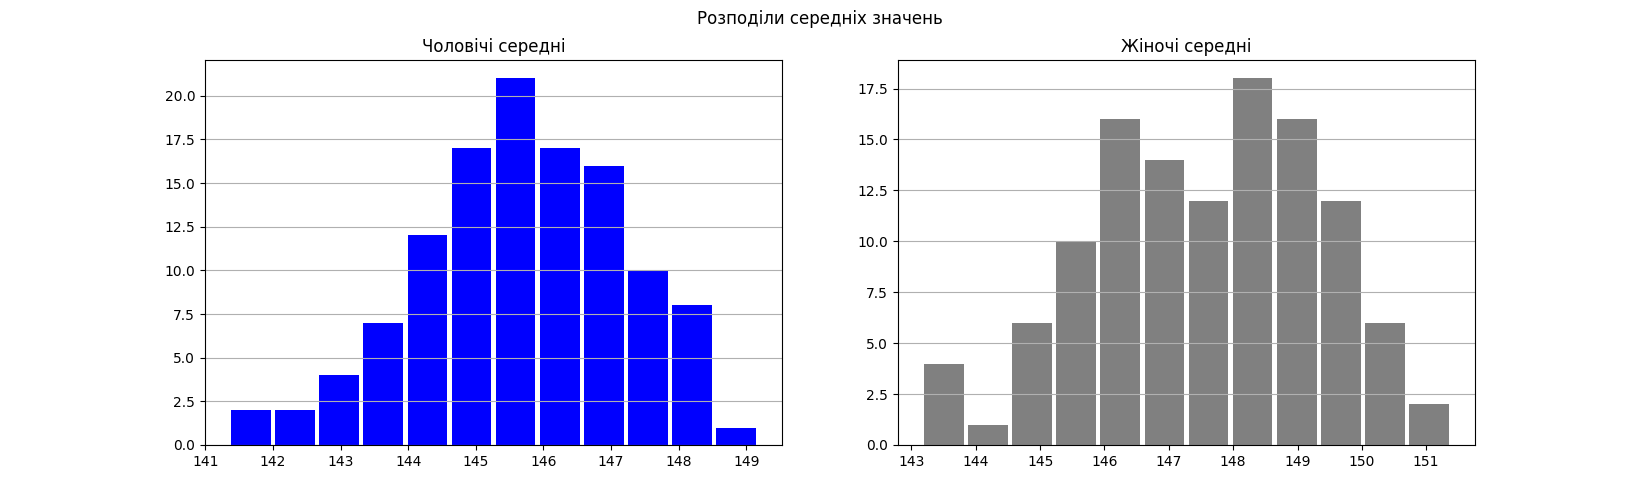
\includegraphics[trim=4cm 0cm 4cm 1cm, clip, width=1\linewidth]{ENG figures/Randomized_means_distribution_m300_N117_v2.png}}
    \caption{Гістограми наборів усереднених результатів ЗНО з англійської мови}
    \label{figure: ENG means data}
\end{figure}

Знову ж таки бачимо, що криві в обох випадках мають схожі риси. Тому висунемо припущення 
(\ref{formula: F-test hypothesis}), що дисперсії цих вибірок однакові:  
\begin{align*}
    &\text{нульова гіпотеза} && H_0: \frac{\sigma_x^2}{\sigma_y^2}=1 \\
    &\text{проти альтернативи} && H_1: \frac{\sigma_x^2}{\sigma_y^2}\neq 1 \nonumber
\end{align*}

При істиності нульової гіпотези статистика критерію Фішера (\ref{formula: F-test statistic}) буде такою:
\begin{equation*}
    \rho\equiv
    \rho(\overline{ x^1}\ldots \overline{x^N},\ \overline{y^1}\ldots \overline{y^N})=\frac{S_Y^2}{S_X^2}
    \sim F\left( N-1,\ N-1 \right)
\end{equation*}

А критерієм перевірки гіпотези слугуватиме правило
\begin{equation*}
    \delta\equiv\delta(\overline{ x^1}\ldots \overline{x^N},\ \overline{y^1}\ldots \overline{y^N})=
    \begin{cases}
        H_1, & \rho\leqslant k^* \text{ або } \rho\geqslant k^{**} \\
        H_0, & \rho\in (k^*,\ k^{**}) \\
    \end{cases}\ ,
\end{equation*}

де значення критичних точок $k^*$ та $k^{**}$ при вказаному рівні значущості $\alpha$ є квантилями розподілу 
Фішера із $(N-1,\ N-1)$ степенями свободи (\ref{formula: F-test criterion values}):
\begin{align*}
    &k^* = f_{\frac{\alpha}{2};\ (N-1,\ N-1)} \\
    &k^{**} = f_{1-\frac{\alpha}{2};\ (N-1,\ N-1)}
\end{align*}

Розіб'ємо усю множину спостережуваних значень на $N=117$ неперетинних множин по $n=300$ елементів у кожній. 
У такому випадку статистична похибка обчислень є малою (детальніше -- на сторінці \pageref{page: ENG percentage point}). 
Наведемо потрібні величини для перевірки гіпотези рівності дисперсій у таблиці нижче:

\vspace{0.8cm}
\begin{table}[H]
    \begin{center}
        \begin{tabular}{||c|c|c|c|c|c||}
            \hline
            $n$ & $N$ & $\alpha$ & $S_X^2$ & $S_Y^2$ \\
            \hline \hline
            300 & 117 & 0.01 & 3.0051 & 2.2830 \\
            \hline
        \end{tabular}
        \caption{Значення шуканих параметрів F-тесту}
        \label{table: ENG F-test}
    \end{center}
\end{table}

Обчислимо значення статистики критерію:
\begin{equation*}
    \rho = \frac{S_Y^2}{S_X^2} = 0.7597
\end{equation*}

Водночас на рівні значущості $\alpha=0.01$ значення критичних точок
\begin{align*} 
   &k^* = f_{\frac{\alpha}{2};\ (N-1,\ N-1)} = f_{0.005;\ (116,\ 116)} = 0.6178 \\
   &k^{**} = f_{1-\frac{\alpha}{2};\ (N-1,\ N-1)} = f_{0.995;\ (116,\ 116)} = 1.6187
\end{align*}

\subsubsection{Висновок}
\label{page: ENG dispersion hypothesis}

Оскільки значення статистики критерію $\rho$ входить у проміжок $(0.6178,\ 1.6187)$, то згідно критерію 
на рівні значущості $\alpha=0.01$ нульова гіпотеза $H_0: \sigma_x^2=\sigma_y^2$ приймається. 
Для подальших міркувань введемо таке позначення: $\sigma_x^2=\sigma_y^2=\sigma^2$.

\subsection*{Побудова довірчого інтервалу для різниці мат. сподівань}
\addcontentsline{toc}{subsection}{Побудова довірчого інтервалу для різниці математичних сподівань}

Аналогічним чином в результаті нормалізації початкових даних та перевірки гіпотези рівності дисперсій 
отримуємо такі дві вибірки: 
\begin{align}
    &\overline{X^1}\ldots \overline{X^N}\sim N(\mu_x,\tfrac{1}{n}\sigma^2) && \text{середні результати чоловіків,} \label{formula: ENG ND X} \\
    &\overline{Y^1}\ldots \overline{Y^N}\sim N(\mu_y,\tfrac{1}{n}\sigma^2) && \text{середні результати жінок,} \label{formula: ENG ND Y}
\end{align}

при цьому
\[ \overline{X^i}=\frac{1}{n}\sum\limits_{j=1}^nX^i_j,\ 
   \overline{Y^i}=\frac{1}{n}\sum\limits_{j=1}^nY^i_j,\ i=\overline{1,N} \]

Спробуємо оцінити, в якому інтервалі лежить значення різниці середніх балів для вибірок результатів ЗНО з 
англійської мови чоловіків та жінок. Виконавши перетворення, які наведенні на сторінці \pageref{page: seaching central statistic}, 
таким самим чином отримаємо шукану центральну статистику $G$ (\ref{formula: G central statistic}) для параметра $\theta=\mu_y-\mu_x:$
\begin{equation*}
    G=\left( (\overline{Y}-\overline{X})-\theta \right)\cdot \sqrt{\frac{N}{S_X^2+S_Y^2}}
    \sim t\left[ 2(N-1) \right]
\end{equation*}

Побудуємо довірчий інтервал рівня довіри $\gamma:$
\begin{equation*}
    \gamma \overset{\mathrm{def}}{=}P(g_1<G<g_2)=\int\limits_{g_1}^{g_2}f_G(x)\ dx
\end{equation*}

В силу симетричності розподілу Ст'юдента, найкоротший центральний довірчий інтервал матиме вид:
\begin{equation*}
    \gamma = P(g_1<G<g_2)=P(|\, G\, |<g),
\end{equation*}

де значення $g$ є квантилем рівня $\frac{1+\gamma}{2}$ розподілу Ст'юдента із $2(N-1)$ степенями свободи 
(Рис. \ref{figure: t interval}), тобто
\begin{equation}
    \gamma = P\left(
        -t_{\tfrac{1+\gamma}{2};\ 2(N-1)} < 
        \left((\overline{Y}-\overline{X})-\theta\right)\cdot \sqrt{\frac{N}{S_X^2+S_Y^2}} < 
        t_{\tfrac{1+\gamma}{2};\ 2(N-1)}
    \right) \label{formula: ENG trusted interval}
\end{equation}

Останнім кроком вкажемо конкретні значення усіх необхідних величин:

\vspace{0.8cm}
\begin{table}[H]
    \begin{center}
        \begin{tabular}{||c|c|c|c|c|c|c||}
            \hline
            $n$ & $N$ & $\gamma$ & $g=t_{0.975;\ 232}$ & $S_X^2$ & $S_Y^2$ & $\overline{Y}-\overline{X}$ \\
            \hline \hline
            300 & 117 & 0.95 & 1.97 & 3.0051 & 2.2830 & 1.9380 \\
            \hline
        \end{tabular}
        \caption{Значення параметрів для довірчого інтервалу різниці середніх}
        \label{table: ENG t interval}
    \end{center}
\end{table}

Підставивши у вираз (\ref{formula: ENG trusted interval}) значення, які наведені у таблиці вище, отримаємо такий довірчий 
інтервал для параметра $\theta=\mu_y-\mu_x$:
\begin{equation}
    P(1.52 < \theta < 2.36)=0.95 \label{formula: calculated ENG trusted interval}
\end{equation}

\subsubsection{Висновок}

Отримано довірчий інтервал рівня довіри $\gamma=0.95$ для величини різниці середніх значень 
оцінок з англійської мови вибірок результатів чоловіків та жінок: $(1.52,\ 2.36)\ni \mu_y-\mu_x$. Оскільки 
у вказаному проміжку немає нульового значення, гіпотезу про нерозрізнюваність середніх можна відхилити. 

Можемо стверджувати, що при порівнянні результатів чоловіка та жінки оцінка з англійської мови у жінки буде 
більшою за оцінку у чоловіка на бал у $1.94\pm 0.42$ пункти, при цьому в середньому у п'яти зі ста таких 
порівнянь вказане наближення може бути хибним.

\subsection{Побудова довірчого інтервалу для значення дисперсії}

Наостанок знову віднайдемо проміжок можливих значень дисперсії нормованих вибірок 
(\ref{formula: ENG ND X})-(\ref{formula: ENG ND Y}). В силу прийняття гіпотези рівності дисперсій 
із оригінальних наборів
\begin{align*}
    &\overline{X^1}\ldots \overline{X^N}\sim N(\mu_x,\tfrac{1}{n}\sigma^2) && \text{середні результати чоловіків} \\
    &\overline{Y^1}\ldots \overline{Y^N}\sim N(\mu_y,\tfrac{1}{n}\sigma^2) && \text{середні результати жінок}
\end{align*}

аналогічними кроками (сторінка \pageref{page: seaching central statistic}) можна сформувати 
випадкову величину (формула \ref{formula: eta}) розподілу хі-квадрат із $\left[ 2(N-1) \right]$ степенями свободи, 
при цьому для параметра дисперсії $\frac{1}{n}\sigma^2$ ця величина відіграватиме роль центральної статистики:
\begin{equation}
    G\equiv\frac{(N-1)}{\sigma^2/n}\left( S_X^2+S_Y^2 \right)\sim \chi^2\left[ 2(N-1) \right]
\end{equation}

А тоді довірчий інтервал рівня довіри $\gamma$ матиме вид:
\begin{equation}
    \gamma \overset{\mathrm{def}}{=} P(g_1<G<g_2)=\int\limits_{g_1}^{g_2}f_G(x)\ dx
\end{equation}

Значення $g_1$ та $g_2$ (Рис. \ref{figure: chi interval}) є квантилями рівнів $\frac{1-\gamma}{2}$ та 
$\frac{1+\gamma}{2}$ розподілу хі-квадрат із $\left[ 2(N-1) \right]$ степенями свободи:
\begin{equation*}
    g_1=\chi^2_{\tfrac{1-\gamma}{2};\ 2(N-1)},\  
    g_2=\chi^2_{\tfrac{1+\gamma}{2};\ 2(N-1)}   
\end{equation*}

Підставляючи отримані результати, матимемо такий ймовірнісний вираз:
\begin{equation}
    \gamma = P\left( 
        \chi^2_{\tfrac{1-\gamma}{2};\ 2(N-1)} < 
        \frac{(N-1)}{\sigma^2/n}\left( S_X^2+S_Y^2 \right) < 
        \chi^2_{\tfrac{1+\gamma}{2};\ 2(N-1)} 
    \right) \label{formula: ENG chi trusted interval}
\end{equation}

На завершення вкажемо конкретні значення усіх необхідних величин:

\vspace{0.8cm}
\begin{table}[H]
    \begin{center}
        \begin{tabular}{||c|c|c|c|c|c|c||}
            \hline
            $n$ & $N$ & $\gamma$ & $g_1=\chi^2_{0.025;\ 232}$ & $g_2=\chi^2_{0.975;\ 232}$ & $S_X^2$ & $S_Y^2$ \\
            \hline \hline
            300 & 117 & 0.95 & 191.71 & 276.08 & 3.0051 & 2.2830 \\
            \hline
        \end{tabular}
        \caption{Значення параметрів для довірчого інтервалу дисперсії}
        \label{table: ENG chi interval}
    \end{center}
\end{table}

Підставивши у вираз (\ref{formula: ENG chi trusted interval}) наведені вище значення, отримаємо 
такий довірчий інтервал для параметра $\frac{1}{n}\sigma^2:$
\begin{equation*}
    P(2.22\ < \frac{\sigma^2}{n} <\ 3.20)=0.95
\end{equation*}

\subsubsection{Висновок}

Тож для сформованих нормально розподілених вибірок (\ref{formula: ENG ND X})-(\ref{formula: ENG ND Y}) 
значення дисперсії в середньому лише у п'яти елементів вибірки зі ста буде виходити за межі проміжку від 
$2.22$ до $3.20$ балів.

\subsection{Статистична похибка обчислень}
\label{page: ENG percentage point}

Статистичною похибкою обчислень називатимемо найменшу величину $\Delta$ відхилення різниці вибіркових 
середніх від істинного значення різниці математичних сподівань заданих вибірок 
(\ref{formula: ENG ND X})-(\ref{formula: ENG ND Y}) з щонайменшою ймовірністю у $95\%$. 
Тобто шукана похибка $\Delta$ обчислюватиметься як така ймовірність:
\begin{equation*}
    P\left(\ \left| (\overline{Y}-\overline{X})-(\mu_y-\mu_x) \right| \leqslant \Delta\ \right)\geqslant 0.95
\end{equation*}

Виконавши аналогічні міркування, які наведені на сторінці \pageref{page: UKR percentage point}, отримаємо, 
що величина похибки $\Delta$ виражатиметься через квантиль рівня $0.975$ розподілу Ст'юдента з 
$\left[ 2(N-1) \right]$ степенями свободи:
\begin{equation}
    \Delta \geqslant t_{0.975;\ 2(N-1)} \cdot \sqrt{\frac{S_X^2+S_Y^2}{N}}
\end{equation}

Таблиця необхідних значень виглядатиме так:

\vspace{0.8cm}
\begin{table}[H]
    \begin{center}
        \begin{tabular}{||c|c|c|c||}
            \hline
            $N$ & $t_{0.975;\ 232}$ & $S_X^2$ & $S_Y^2$ \\
            \hline \hline
            117 & 1.97 & 3.0051 & 2.2830 \\
            \hline
        \end{tabular}
        \caption{Значення параметрів для обчислення статистичної похибки}
        \label{table: ENG percentage point}
    \end{center}
\end{table}

Тож остаточно найменша величина відхилення $\Delta = 0.42$, а тоді початкова ймовірнісна нерівність матиме вид:
\begin{equation*}
    P\left(\ \left| (\overline{Y}-\overline{X})-(\mu_y-\mu_x) \right| \leqslant 0.42\ \right)\geqslant 0.95
\end{equation*}

\subsubsection{Висновок}

Для встановлених значень $n=300$ й відповідно $N=117$ статистична похибка відхилення різниці вибіркових 
середніх від істинного значення різниці математичних сподівань складає $\Delta = 0.42$ бала з ймовірністю, 
більшою за $95\%$. Можемо стверджувати, що обчислення за такого значення похибки мають високу точність, 
оскільки величина $\Delta = 0.42$ є лише $0.2\%$ від можливих $200$ балів за результат тесту.